\pagenumbering{arabic}
\section{工程概况}
\subsection{施工组织设计编制基本原则}

施工组织设计按照编制对象,可分为施工组织总设计、单位工程施工组织设计。
施工组织设计应包括编制依据、工程概况、施工部署、施工准备与资料配置计划、
施工进度计划、主要施工方法、施工管理措施、施工现场平面布置等主要内容;
施工组织设计的编制必须遵循工程建设程序,并符合下列原则:\\

\begin{itemize}

    \item [1)] 符合国家有关法律法规、现行规范,符合地方规程、行业标准的要求;

    \item [2)] 满足建筑施工合同或招标文件中关于建筑工程进度、质量、环境保护、职业健康、安全、工程造价等工程管理目标的要求;

    \item [3)] 积极开发、推广运用新技术、新工艺、新材料、新设备;

    \item [4)] 坚持科学的施工程序和合理的施工顺序,做到资源的优化组织和合理配置,采用流水施工和网络计划的方法,实现均衡施工,努力实现科学、合理的经济技术指标;

    \item [5)] 积极响应国家关于低碳、节能、环保方面的方针、政策;采取先进的技术和管理措施,推广建筑节能和绿色施工。

    \item [6)] 与建筑施工单位质量、环境、职业健康安全、项目管理规范四合一标准的有效结合,贯彻质量、环境、职业健康安全管理国家管理规范的要求;

\end{itemize}

\subsection{施工组织设计编制程序}

施工组织设计的编制程序流程图见图 \ref{fig:c1f1}

\begin{figure}[thbp!]
    \centering
    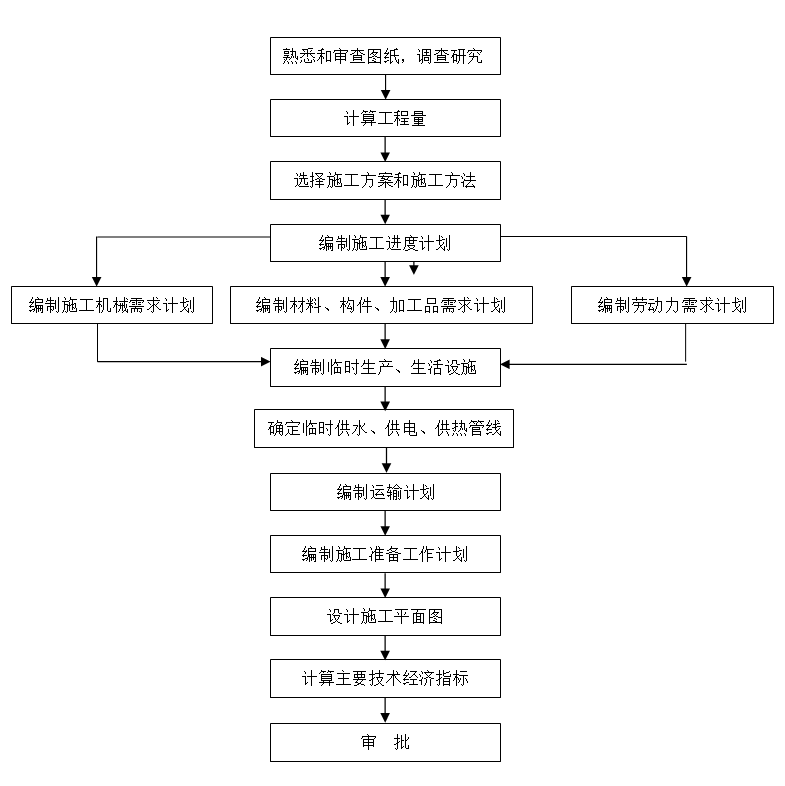
\includegraphics[width=0.5\linewidth]{figure/01.png}
    \caption{单位工程施工组织设计编制程序}
    \label{fig:c1f1}
    \end{figure}

\subsection{指导方针及编制依据}

\subsubsection{指导方针}

(1) 主要指导方针\\

为保证在计划工期内圆满地完成施工任务,本施工组织设计的主要指导方针是“服务至上,质量争先,科技先导,管理一流”。\\

(2) 科学组织、精心施工\\

组建一个高效团结的工程项目部和一支技术熟练、作风过硬的施工队伍,运用先进科学的现代化管理手段,
调动企业人力、物力、机械设备等各方面的优势资源,精心组织,与甲方、监理、各专业施工单位、工种密切配合,
根据工期进度要求,从图纸设计、现场测量、材料组织、现场施工、质量检验实行流水节拍式循环作业,
确保工程顺利按时完工。\\

(3) 质量第一、安全至上\\

制定严格的质量保证制度,充分考虑国家现行有关施工质量验收规范、标准和规定的要求,
从人员、材料、机械、环境等方面采取保证质量的措施,实施全员质量管理,确保工程质量达到预定目标。
建立完善的安全保证体系,制定严格的安全管理制度,遵守有关施工安全、防火、环卫的法律、法规,
坚决杜绝重大伤亡事故的发生,保证安全施工、文明施工。\\

(4) 科技先导、争创一流\\

采用先进的施工技术,科学合理地确定施工方案,在确保施工质量和效果的前提下,提高材料利
用率和工作效率,降低施工成本,提高经济效益。\\



\subsubsection{编制依据}

施工组织设计应以下列内容为主要编制依据:\\

\begin{itemize}

    \item [1)] 与建筑工程有关的法律、法规和相关文件;

    \item [2)] 国家现行有关标准、规范和技术经济指标;

    \item [3)] 工程所在地的行政主管部门的管理要求;

    \item [4)] 建筑施工行业相关的的质量、环境、职业健康安全管理体系管理规范的要求;

    \item [5)] 工程施工合同及招投标文件;

    \item [6)] 工程设计文件

    \item [7)] 项目周边环境、现场条件、工程地质和水文、气象等自然条件;

    \item [8)] 与工程项目施工有关的资源供应、生产要素配置情况;

    \item [9)] 施工单位的生产能力、机具设备状况、技术水平等等。
    
\end{itemize}


\subsection{工程概况}
\subsection{建筑设计概况}
\subsection{结构设计概况}
\subsection{气象地质特点}

